\documentclass[tikz,border=10pt]{standalone}
\usetikzlibrary{angles}
\begin{document}
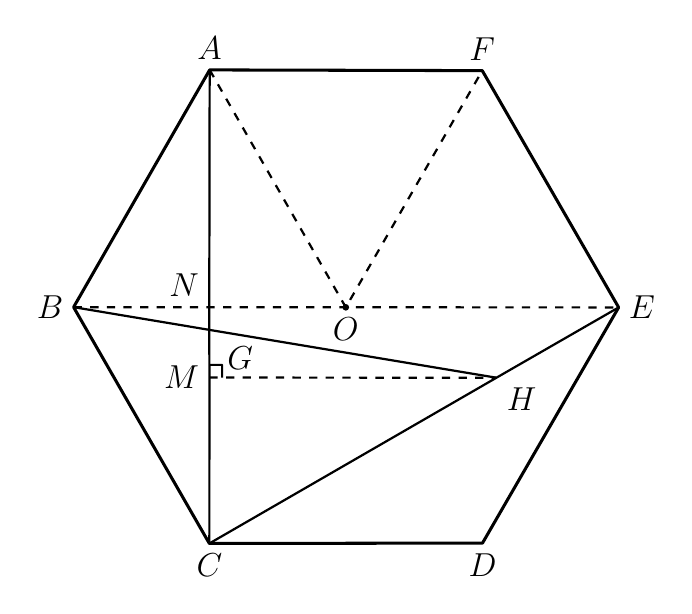
\begin{tikzpicture}[line width=0.8pt, line join=round,
  lbl/.style={font=\fontsize{11.5}{13.8}\selectfont}]
\coordinate (A) at (-1.734,3.022);
\coordinate (B) at (-3.462,0.009);
\coordinate (C) at (-1.738,-2.992);
\coordinate (D) at (1.731,-2.987);
\coordinate (F) at (1.728,3.013);
\coordinate (G) at (-1.739,-0.279);
\coordinate (H) at (1.908,-0.887);
\coordinate (M) at (-1.737,-0.885);
\coordinate (N) at (-1.739,0.007);
\coordinate (O) at (-0.005,0.007);




\coordinate (E) at (3.460,0.006);


\draw[line width=1.1pt] (A) -- (B) -- (C) -- (D) -- (E) -- (F) -- cycle;


\draw (A) -- (N) -- (G) -- (M) -- (C);


\draw[dashed] (B) -- (N) -- (O) -- (E);


\draw (B) -- (G) -- (H);
\draw (C) -- (H) -- (E);


\draw[dashed] (M) -- (H);


\draw[dashed] (A) -- (O) -- (F);


\draw pic[draw, angle radius=0.161cm] {right angle=A--M--H};

\fill (O) circle (1.200pt);


\node[above, lbl] at (A) {$A$};
\node[above, lbl] at (F) {$F$};
\node[left, lbl] at (B) {$B$};
\node[right, lbl] at (E) {$E$};
\node[below, lbl] at (C) {$C$};
\node[below, lbl] at (D) {$D$};
\node[above left, lbl] at (N) {$N$};

\node[below right, xshift=0.10cm, yshift=-0.08cm, lbl] at (G) {$G$};
\node[below, lbl] at (O) {$O$};
\node[below right, lbl] at (H) {$H$};
\node[left, lbl] at (M) {$M$};
\end{tikzpicture}
\end{document}